\begin{frame}
	\myheading{Module 8.3 :  True error and Model complexity}
\end{frame}

\begin{frame}
	\begin{itemize}
		\justifying
		\setlength\itemsep{1em}
		\item[]<1-> Using Stein's Lemma (and some trickery) we can show that\\
		      \begin{align*}
		      	\frac{1}{n}\sum_{i=1}^{n}\varepsilon_i(\hat{f}(x_i)-f(x_i))=\frac{\sigma^2}{n}\sum_{i=1}^{n}\frac{\partial\hat{f}(x_i)}{\partial y_i} 
		      \end{align*}
		      \item<2->When will $\frac{\partial\hat{f}(x_i)}{\partial y_i}$ be high? When a small change in the observation causes a large change in the estimation($\hat{f}$)
		      \item<3->Can you link this to model complexity?
		      \item<4->Yes, indeed a complex model will be more sensitive to changes in observations whereas a simple model will be less sensitive to changes in observations
		      \item<5->Hence, we can say that\\
		      true error = empirical train error + small constant + $\Omega$(model complexity)
	\end{itemize}
\end{frame}

\begin{frame}
	\begin{columns}
		\begin{column}{0.4\textwidth}
			\begin{figure}
				\includegraphics<2>[width=0.9\linewidth]{images/1a.png}
				\includegraphics<3>[width=0.9\linewidth]{images/1b.png}
				\includegraphics<4>[width=0.9\linewidth]{images/1d.png}
			\end{figure}
		\end{column}
		\begin{column}{0.4\textwidth}
			\begin{itemize}\justifying
				\item Let us verify that indeed a complex model is more sensitive to minor changes in the data
				      \item<2-> We have fitted a simple and complex model for some given data
				      \item<3-> We now change one of these data points	
				      \item<4-> The simple model does not change much as compared to the complex model  
			\end{itemize}
		\end{column}
	\end{columns}
	
\end{frame}

%%%%%%%%%%%%%%%%%%%%%%%%%%%%%%%%%%%%%%%%%%%%%%%%%%%%%%%
\begin{frame}
	\begin{itemize}
		\justifying
		\setlength\itemsep{1em}
		\item<1->Hence while training, instead of minimizing the training error $\mathscr{L}_{train}(\theta)$ we should minimize
		\begin{align*}
			\min\limits_{w.r.t\ \theta} \mathscr{L}_{train}(\theta) + \Omega(\theta) = \mathscr{L}(\theta)
		\end{align*}
		\item<2->Where $\Omega(\theta)$ would be high for complex models and small for simple models
		\item<3->$\Omega(\theta)$ acts as an approximate for $\frac{\sigma^2}{n}\sum_{i=1}^{n}\frac{\partial\hat{f}(x_i)}{\partial y_i}$
		\item<4->This is the basis for all regularization methods
		\item<5->We can show that $l_1$ regularization, $l_2$ regularization, early stopping and injecting noise in input are all instances of this form of regularization.
	\end{itemize}
\end{frame}
%%%%%%%%%%%%%%%%%%%%%%%%%%%%%%%%%%%%%%%%%%%%%%%%%%%%%%
\begin{frame}
	\centering
	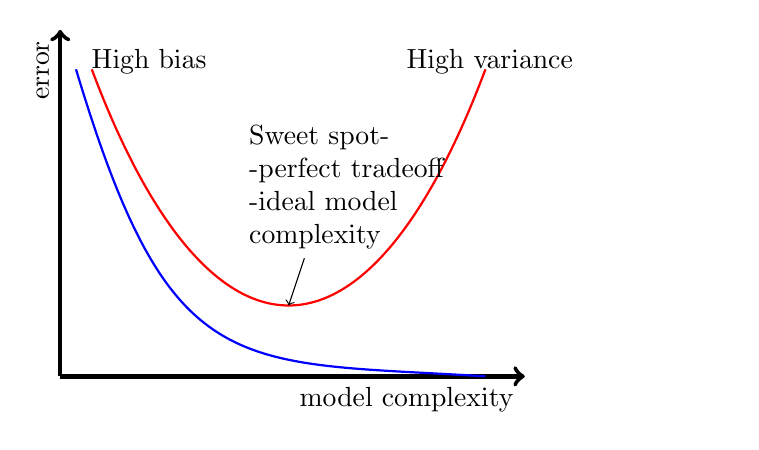
\begin{tikzpicture}
	\draw[->,ultra thick] (4.1,-0.9)--(10,-0.9) node[below left]{model complexity};
	\draw[->,ultra thick] (4.1,-0.9)--(4.1	,3.5) node[above left,rotate=90]{error};
					
	\onslide<5->{\draw[blue,thick] (4.3,3) .. controls (5.5,-1) and (6.3,-0.7) .. (9.5,-0.9);}
	\onslide<6->{\draw[red,thick] (4.5,3) .. controls (6,-1) and (8,-1) .. (9.5,3);}
	\onslide<7->{\node[text width=4cm] at (6.5,3.1) {High bias};}
	\onslide<8->{\node[text width=4cm] at (10.5,3.1) {High variance};}
	\onslide<9->{\node[text width=3cm] at (8,1.5) {Sweet spot-\\-perfect tradeoff \\ -ideal model\\ complexity};}
	\onslide<9->{\draw[->] (7.2,0.6)--(7,0);}			
\end{tikzpicture}
\end{frame}
		
\begin{frame}
	\begin{columns}
		\column{0.4\textwidth}
		\begin{overlayarea}{\textwidth}{\textheight}
			\justifying
			\begin{itemize}
				\item<1-> Why do we care about this bias variance tradeoff and model complexity?
			\end{itemize}

		\end{overlayarea}
		\column{0.6\textwidth}
		\begin{overlayarea}{\textwidth}{\textheight}
			\begin{itemize}
				\justifying
				\item<2->  Deep Neural networks are highly complex models.
				\item <3-> Many parameters, many non-linearities.
				\item <4-> It is easy for them to overfit and drive training error to 0.
				      \item<5->  Hence we need some form of regularization.
			\end{itemize}
		\end{overlayarea}
	\end{columns}
\end{frame}
		
%%%%%%%%%%%%%%%%%%%%%%%%%%%%%%%%%%%%%%%%%%%%%%%%%%%%%%%%%%%%
\begin{frame}
	\vspace{4em}
	\begin{overlayarea}{\textwidth}{\textheight}
		\begin{block}{Different forms of regularization}
			\begin{itemize}
				%\renewcommand\label itemi{--}
				\item<1-> $l_2$ regularization
				\item<2-> Dataset augmentation
				\item<3-> Parameter Sharing and tying
				\item<4-> Adding Noise to the inputs 
				\item<5-> Adding Noise to the outputs
				\item<6-> Early stopping
				\item<7-> Ensemble methods
				\item<8-> Dropout
			\end{itemize}
		\end{block}
	\end{overlayarea}
\end{frame}
